\section{Estructuras de contención} % (fold)
\label{sec:estructuras_de_contención}

\question{¿Existe alguna relación analítica entre el FS al vuelco de un muro de gravedad y el valor de la excentricidad de la resultante de fuerzas al c.d.g de la base del mismo ? (Suponer que la única acción desfavorable es el empuje activo y la única favorable el peso)}{
	
}

\question{Citar ventajas e incovenientes de utilizar tablestacas metálicas como elementos de contención de tierras}{
	\begin{minipage}[t]{0.5\textwidth}
	Ventajas:
	\begin{itemize}
		\item Fáciles de manejar (ligeras)
		\item Recuperables (provisionales)
		\item $\exists$ diversos perfiles prefabricados
		\item Muy flexibles
	\end{itemize}
	\end{minipage}%
	\begin{minipage}[t]{0.5\textwidth}
		Inconvenientes:
		\begin{itemize}
			\item Longitud limitada ($<12m$)
			\item Posible corosión (en ambientes agresivos)
			\item No pueden atravesar zonas duras (se doblan)
			\item Dificil control de estanqueidad
			\item Dificil control de la verticalidad en el hincamiento
		\end{itemize}
	\end{minipage}	
}

\question{¿Qué problemas de tipo contructivo pueden presentarse en pantallas hormigonadas \emph{in-situ}?}{
	\begin{enumerate}
		\item Mal control del hormigonado (cavidades dificiles de detectar)
		\item Difícil control de la estanqueidad
		\item Problemas con capas duras (trépano, martillos disminuyen la productividad)
		\item Problemas de estabilidad de paredes de excavación 
		\item Durabilidad del hormigón
		\item Coqueras
		\item Posibilidad de contaminación de las armaduras por contacto con suelos plásticos
	\end{enumerate}
}

\question{Para estabilizar un muro de 30m de longitud, se necesita aplicar una f=50T/ml. Cuántos anclajes serán necesarios si cada anclaje:
\begin{itemize}
	\item Sección de acero: $2 \cdot 10^{-3}m^2$
	\item Límite elástico acero: $2 \cdot 10^{5}T/m^2$
	\item $\varphi_{bulbo}=0.1m$
	\item Longitud del bulbo: 6m
	\item Resistencia al corte unitaria en el contacto bulbo-terreno: $100T/m^2$
	\item FS frente arrancamiento: 1.8
	\item FS frente a rotura de tracción del acero: 1.5
\end{itemize}}{
	Acero:
	\[
		Q_a = \frac{0.9f_{ys}}{\gamma_l \cdot \gamma_y}A_{acero} = 240T
	\]
	Bulbo:
	\[
		Q_b = \frac{\tau}{\gamma_l \cdot \gamma_t}A_l = 104.7T
	\]
	Luego $Q=\min(Q_a,Q_b)$ y $f_{tot}= f \cdot d = 50 \cdot 30 =1500T$
	Así pues:
	\[
		N = \frac{f_{tot}}{Q} \approx 14.3 \Rightarrow N=15
	\]	
}

\question{Se tiene el siguiente muro Figure~\ref{fig:anclaje} con el mecanismo de rotura indicado. Se debe colocar una fila de anclajes a la cota indicada. Dar:
\begin{enumerate}
	\item Inclinación óptima del anclaje
	\item Longitud mínima
\end{enumerate}}{
	\begin{figure}[H]
		\centering
		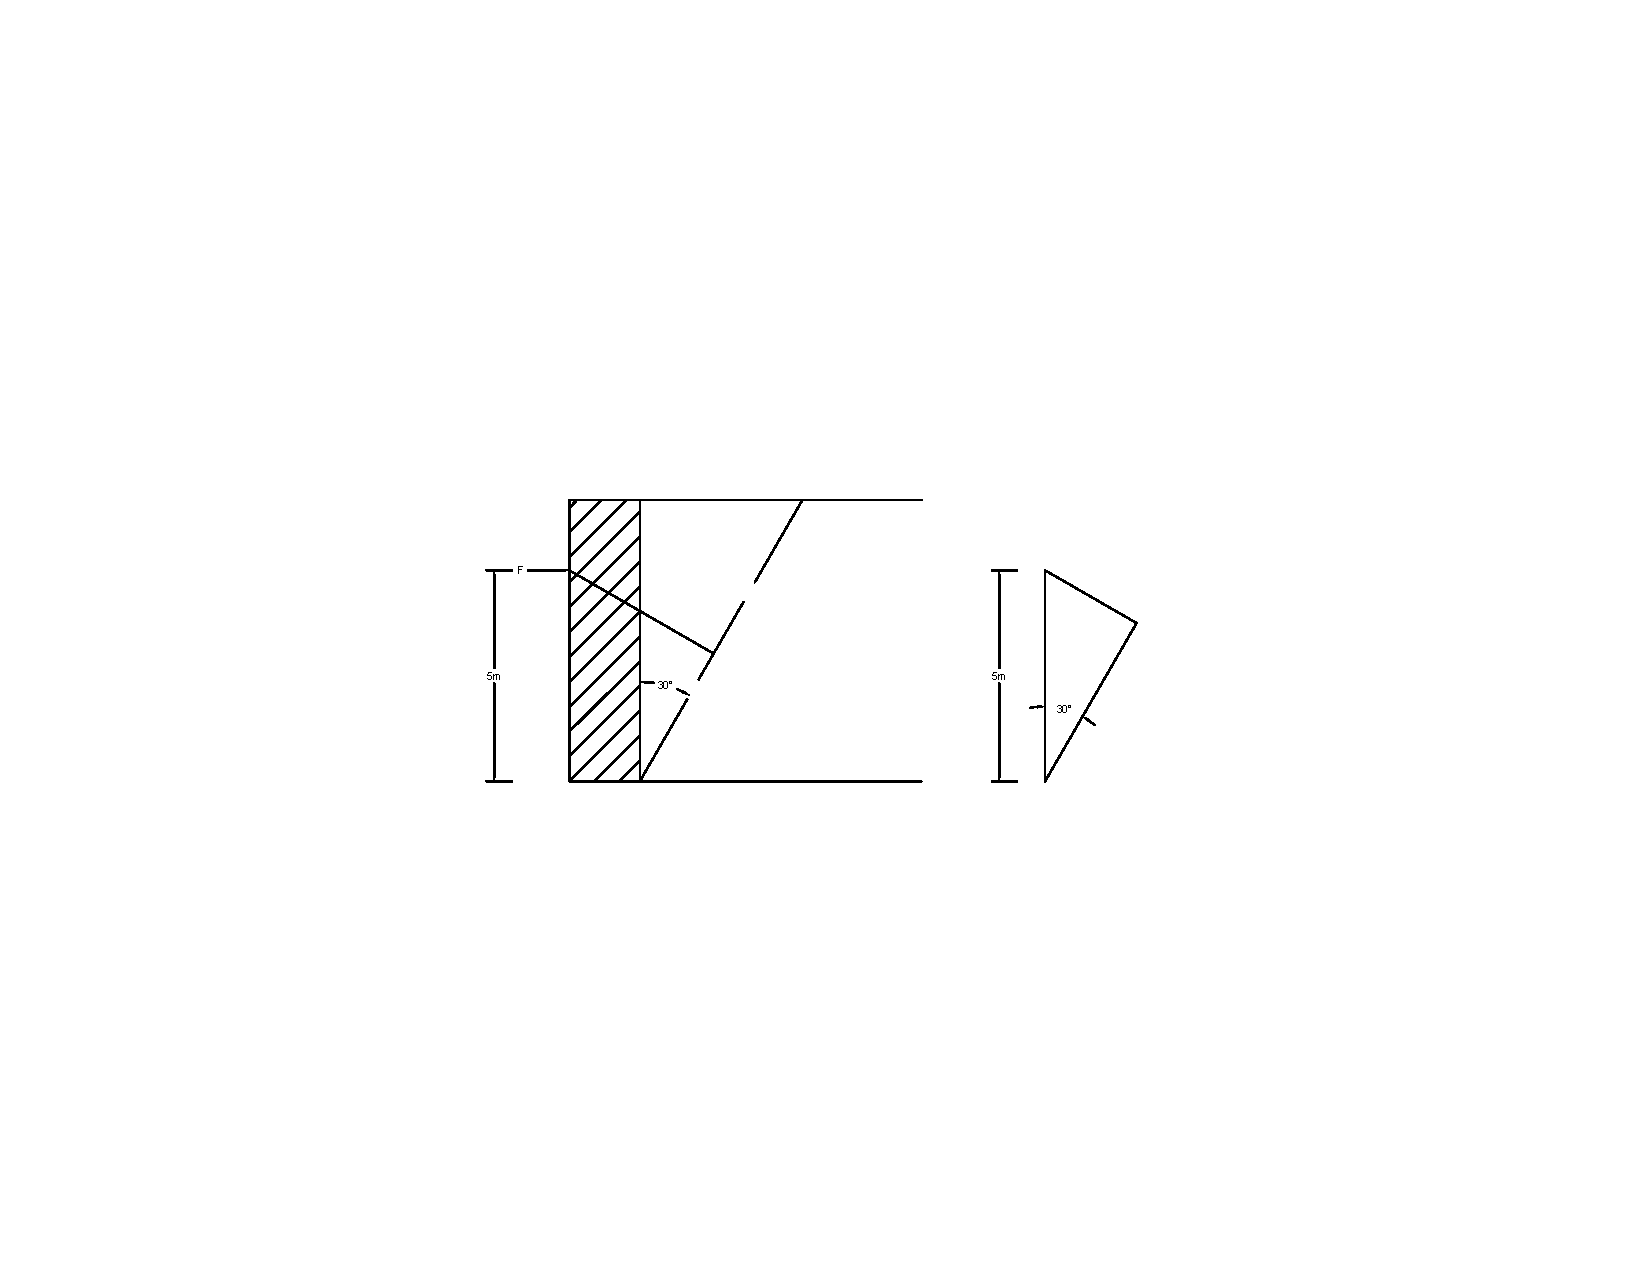
\includegraphics[width=0.5\textwidth]{img/anclaje}
		\caption{Muro}
		\label{fig:anclaje}
	\end{figure}
	Para maximizar su eficiencia han de ser perpendiculares a la superficie de rotura luego por relaciones trigonométricas obtenemos $l>2.5m \Rightarrow l \approx 3m$
}

\question{Calcular la estabilidad frente a deslizamiento del muro de la Figure~\ref{fig:desli}. $\nexists $agua, terreno horizontal, $\delta = 25$}{
	\begin{figure}[H]
		\centering
		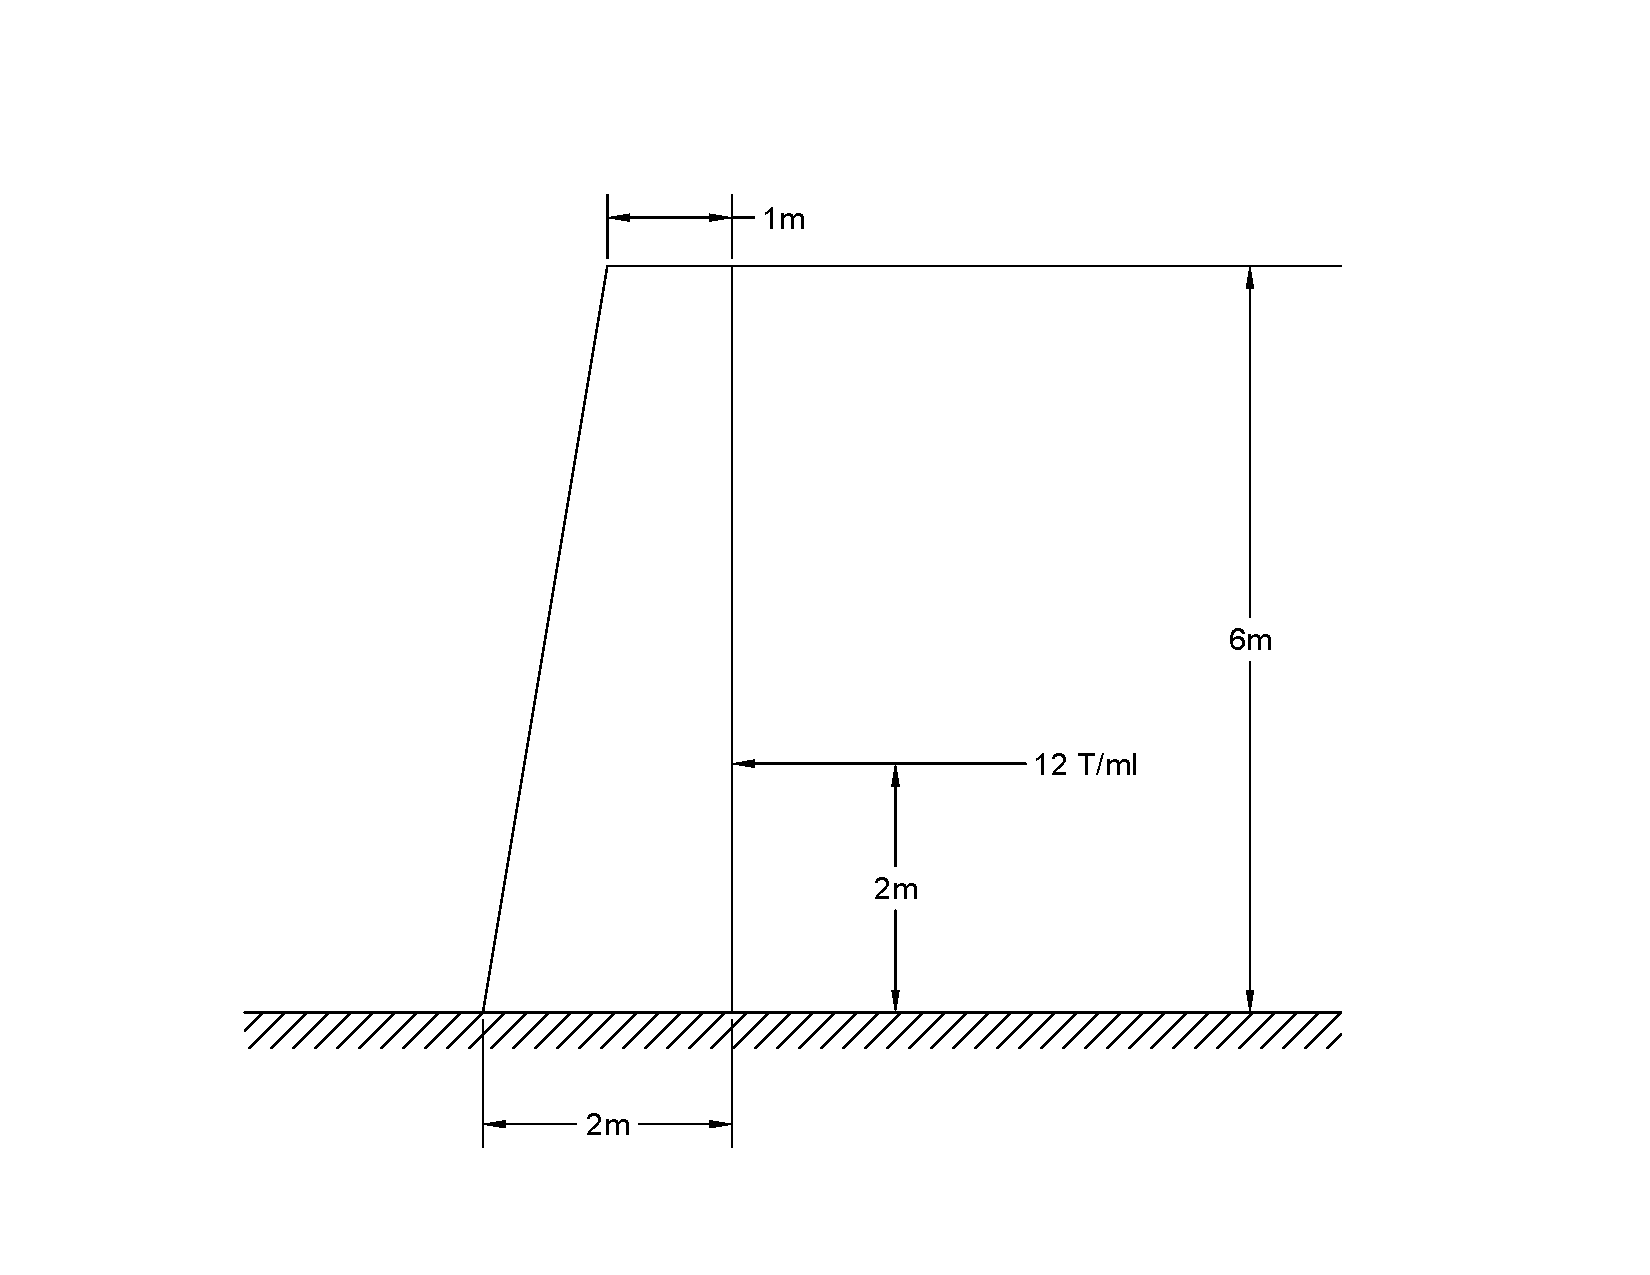
\includegraphics[width=0.9\textwidth]{img/deslizamiento}
		\caption{Muro}
		\label{fig:desli}
	\end{figure}
	\[
		F_d = \frac{F_{res}}{F_{act}} = \frac{N \tan( \delta )}{T} = \frac{W \tan( \delta )}{T} =\frac{9,25 \tan( 25 )}{12} = 0,87
	\]
}

\question{En un acceso subterráneo a una rotonda, se construye el muro-ménsula dibujado en la Figure~\ref{fig:l_empuje}. El terreno es un medio granular de $\phi = 30, \gamma =20KN/m^3$. Su empuje sobre la estructura es de tipo activo. A efectos de predimensionamiento, se considera que el empuje del terreno ($\vec{E}$) es horizontal, actúa en el trasdós ficticio indicado y se calcula mediante la solución de Rankine.
Calcular coeficiente de estabilidad frente al deslizamiento e indicar si la estructura es estable frente a este mecanismo. Para el cálculo se despreciará el peso del hormigón y el empuje activo y pasivo que actúan en las caras verticales del tacón y de la puntera.}{
	\begin{figure}[H]
		\centering
		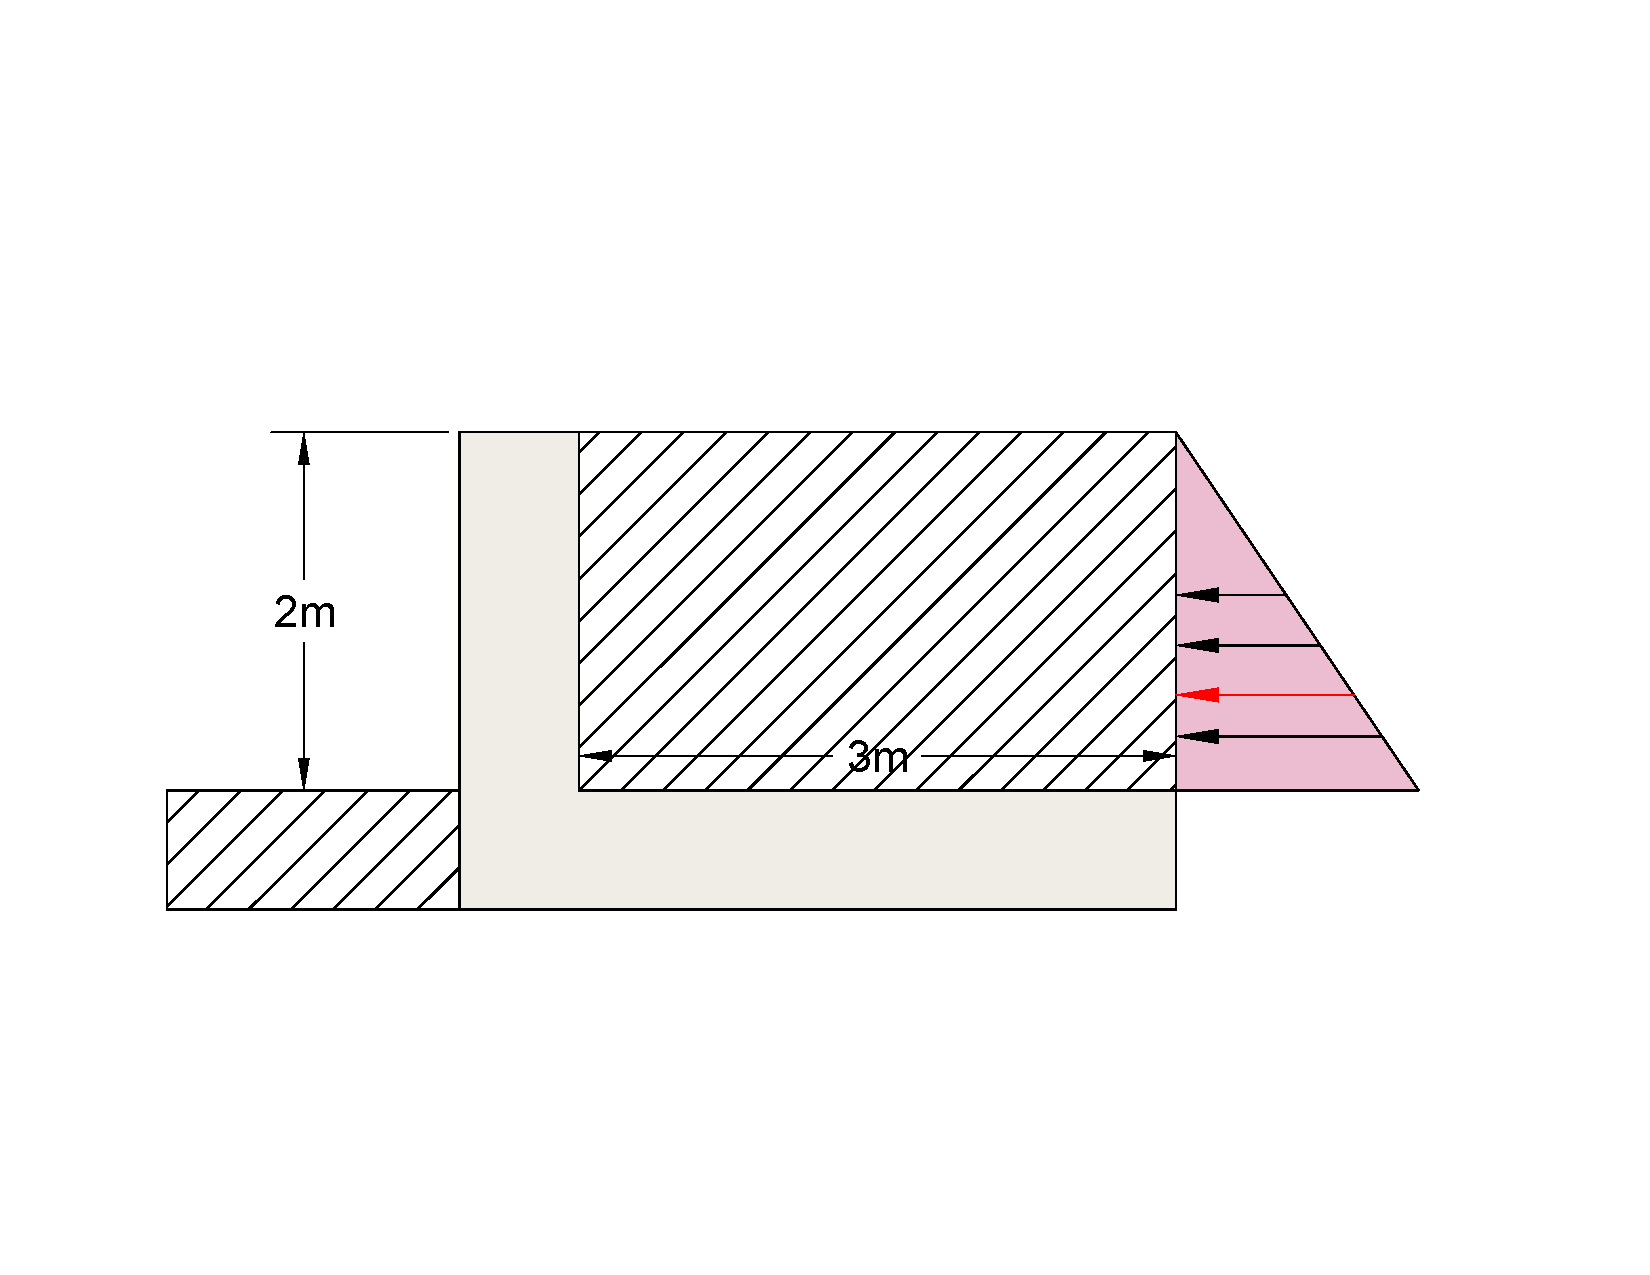
\includegraphics[width=0.9\textwidth]{img/l_empuje}
		\caption{Muro-ménsula}
		\label{fig:l_empuje}
	\end{figure}
}

\question{Calcular el FS frente al deslizamiento en el caso de la estructura de la Figure~\ref{fig:t_empuje}. El empuje de las tierras se cálcula en el trasdós ficticio AB mediante la fórmula del empuje activo de Rankine. La estructura es de hormigón y se considera en el cálculo que no tiene estpeso y no pesa. ¿Es estable la estructura? En el caso negativo, indica una modificación de geometría que mejora la estabilidad frente al deslizamiento.}{
	\begin{figure}[H]
		\centering
		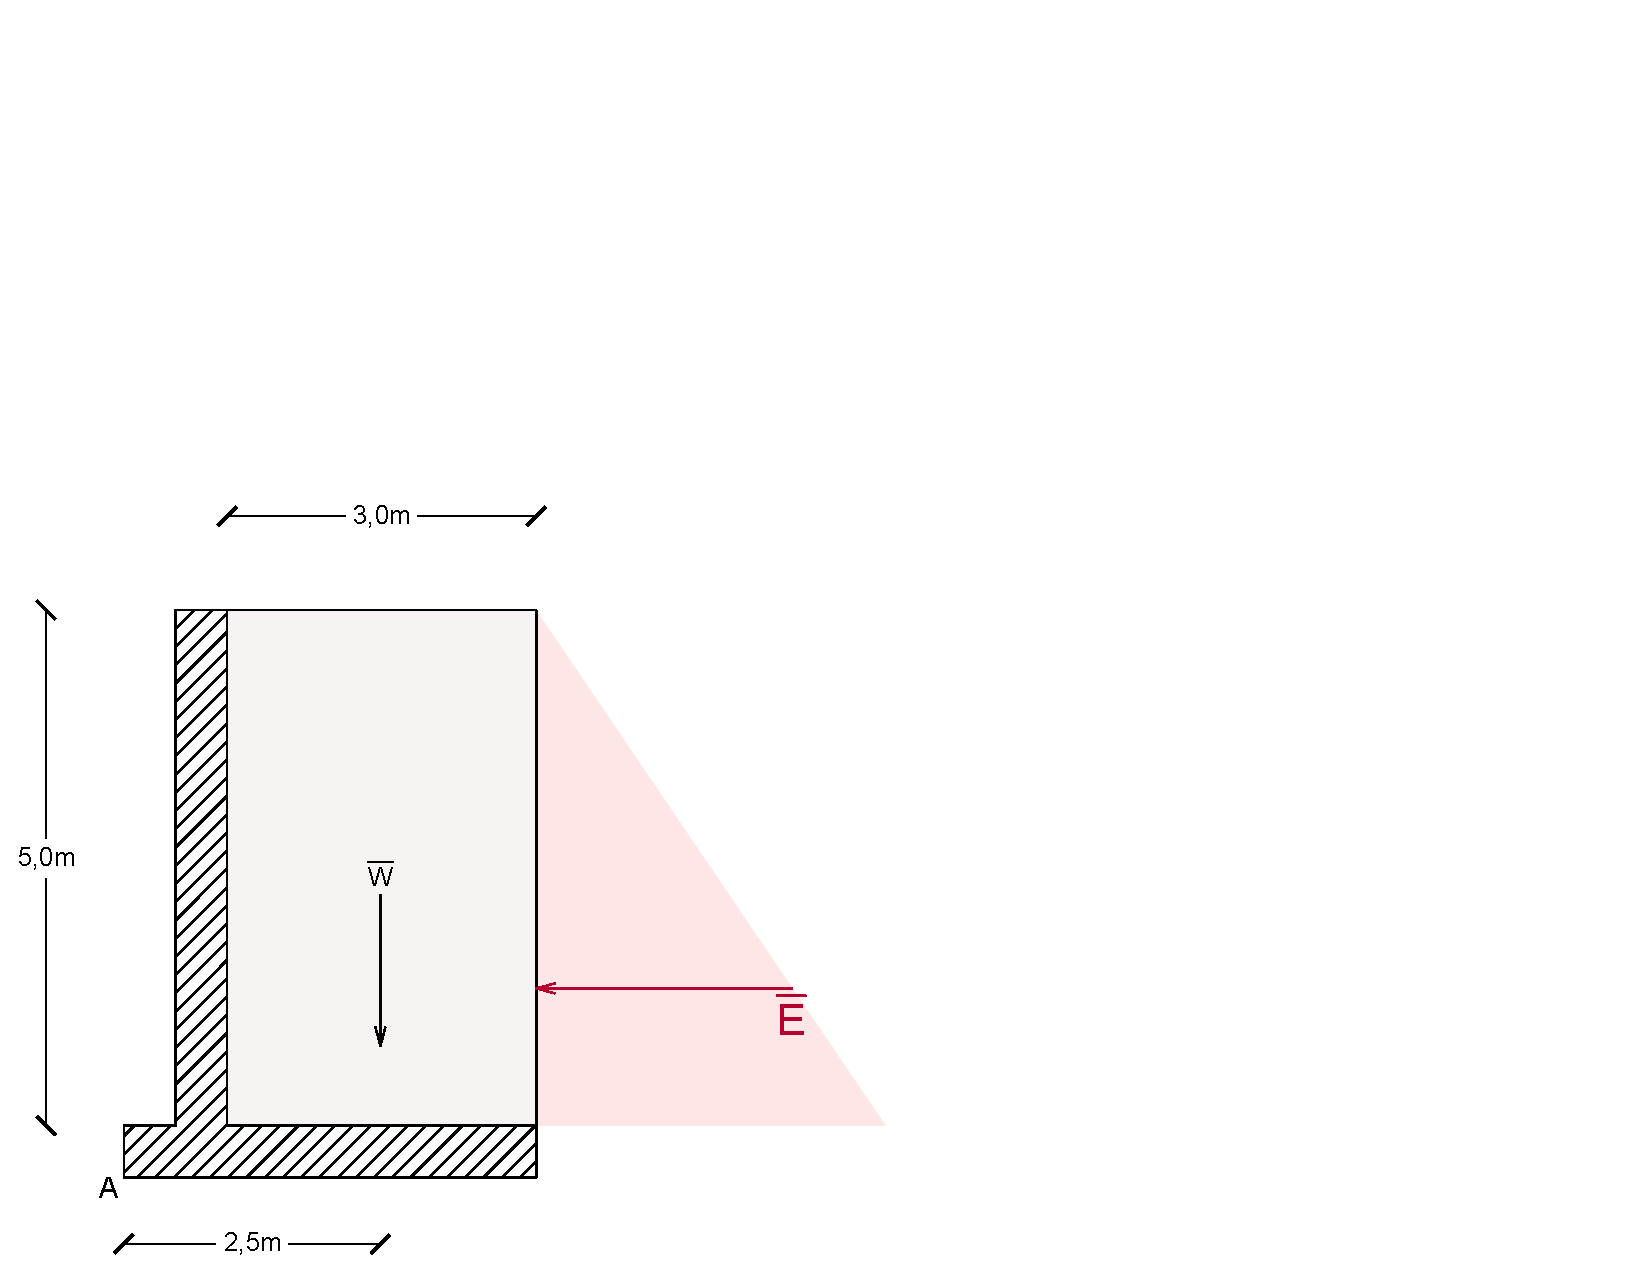
\includegraphics[width=0.9\textwidth]{img/t_section}
		\caption{Muro con llave}
		\label{fig:t_empuje}
	\end{figure}
}

\question{Una pantalla contiene una excavación sumergida. ¿Qué posición de la Figure~\ref{fig:pantalla_nf} es más estable ? }{
	Podemos observar que en la situación 1 los empujes hidrostaticos se compensan pero al ser menor la densidad saturada el empuje tierras resultante es menor ($\gamma_{sat}< \gamma_{dry}$). Luego la situación más favorable es la 1.
	\begin{figure}[H]
		\centering
		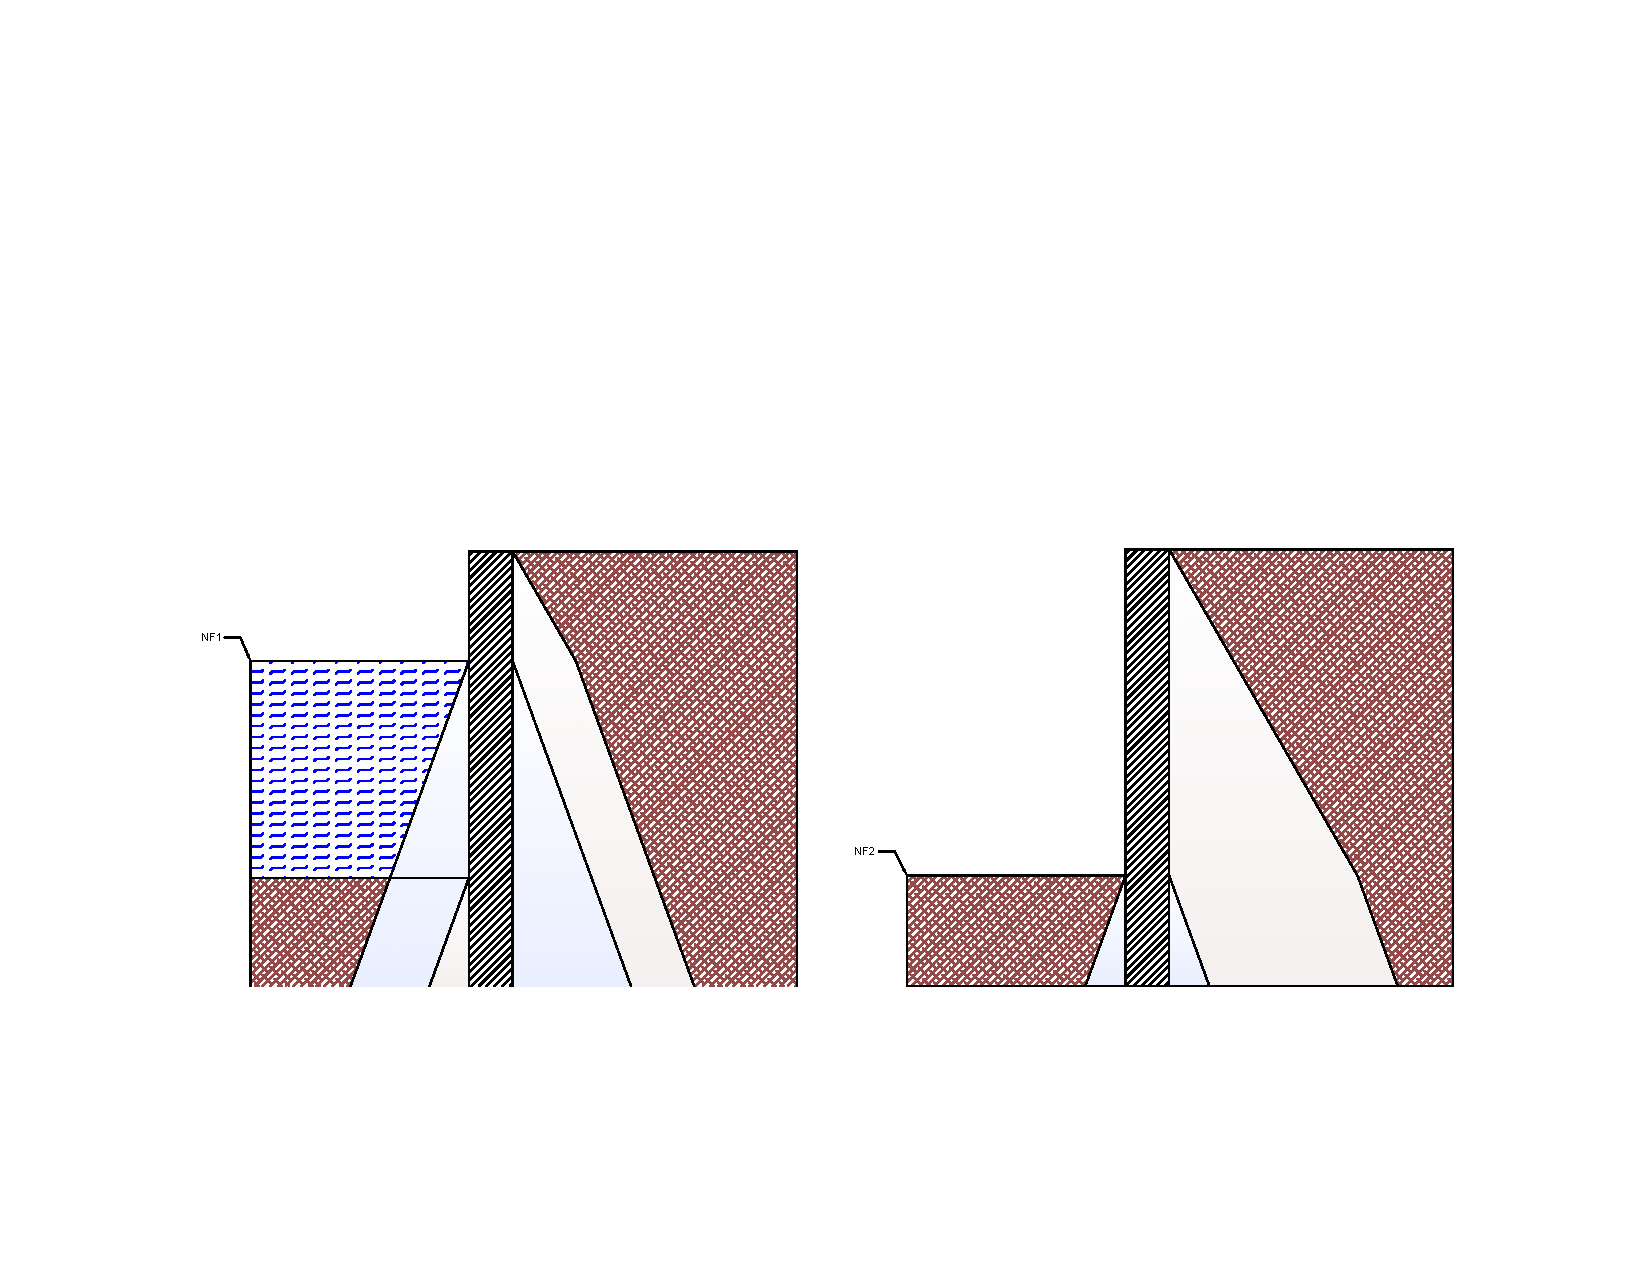
\includegraphics[width=0.9\textwidth]{img/pantalla}
		\caption{Esfuerzos en pantallas en función del nivel freatico.}
		\label{fig:pantalla_nf}
	\end{figure}
}

\question{¿Qué riesgos comporta una mala ejecución de las juntas de hormigonado en el caso de muros de gravedad?}{
	\begin{enumerate}
		\item Son puntos débiles en el muro, por donde podrán fisurarse
		\item Si no respetan su ángulo de diseño (pueden aparecer coqueras)
		\item Daños estéticos (se rompe la unidad visual del muro)
		\item Corrosión de la armadura por infiltración de agua
	\end{enumerate}
}

\question{Un muro en L empieza a fallar a base de girar sobre su puntera. Señala un mínimo de 3 medidas correctoras de carácter urgente}{
	\begin{enumerate}
		\item Descargar el trasdós
		\item Colocar anclajes
		\item Acodarlo
	\end{enumerate}
}

\question{En una estructura de tierra armada. ¿Qué 2 criterios de estabilidad han de cumplirse?}{
	\begin{enumerate}
		\item Rotura a tracción:
		\[
			T_M \leq \frac{1}{F_1}\sigma_r b e
		\]
		\item Adherencia:
		\[
			T_M^{*}\leq \frac{1}{F_2}\int_0^{2a}\mu^* \sigma_v(x)2bdx
		\]

	\end{enumerate}
	Cálculo de la tracción máxima:
	\[
		T_M = \frac{1}{n}\sigma_h \Delta H
	\]
}

% section estructuras_de_contención (end)